\documentclass[iop]{emulateapj}
\usepackage{color}
\usepackage{natbib}
\usepackage{amsmath}
\bibliographystyle{apj}

\newcommand{\vdag}{(v)^\dagger}
\newcommand{\myemail}{eogorma@tcd.ie}

\shorttitle{BETELGEUSE'S WIND ACCELERATION REGION}
\shortauthors{O'GORMAN ET AL.}

\begin{document}

\title{MULTI EPOCH SPATIALLY RESOLVED RADIO OBSERVATIONS OF BETELGEUSE'S WIND ACCELERATION REGION}


\author{Eamon O'Gorman\altaffilmark{1}, Graham M. Harper\altaffilmark{1}, Alexander Brown\altaffilmark{2}, and Anita M. S. Richards\altaffilmark{3}}
\altaffiltext{1}{School of Physics, Trinity College Dublin, Dublin 2, Ireland}
\altaffiltext{2}{Center for Astrophysics and Space Astronomy, University of Colorado, 389 UCB, Boulder, CO 80309, USA}
\altaffiltext{3}{Jodrell Bank Centre for Astrophysics, School of Physics and Astronomy, University of Manchester, Manchester M13 9PL, UK}

%\email{eogorma@tcd.ie}
%\email{graham.harper@tcd.ie}
%\email{alexander.brown@colorado.edu}
%\email{a.m.s.richards@manchester.ac.uk}


\begin{abstract}

Previous VLA observations have only spatially resolved the stellar atmosphere at 0.7\,cm but here we fully resolve the star at all wavelengths between 0.7 and 6.1\,cm. New multi-epoch e-MERLIN data are urgently required.

\end{abstract}

\keywords{Radio continuum: stars --- Stars: supergiants --- Stars: individual ($\rm{\alpha}$ Ori) --- Stars: mass-loss --- Stars: winds, outflows}

\section{INTRODUCTION}
Red supergiants (RSGs) lose mass to the interstellar medium in the form of a massive ($\dot{M} \sim 10^{-7} - 10^{-4}\,M_{\odot}\,\rm{yr}^{-1}$) cool wind, with terminal velocities ($10\lesssim v_{\infty}\lesssim 50\,{\rm{km}}\,\rm{s}^{-1}$) typically less than the photospheric escape velocity  ($v_{\rm{esc}} \sim 100\,\rm{km},\rm{s}^{-1}$). These winds are major contributors of heavy elements to the interstellar medium (ISM) and play a crucial role in stellar evolution \citep{chiosi_1986}, and also in explaining the frequency of supernovae in the galaxy \citep[e.g.,][]{van_loon_2010}. Despite their importance, the mechanisms responsible for the formation of these winds in late K and early M-type RSGs remain largely unknown. Dust is observed too far from the star to play a significant role in the mass-loss process \citep{danchi_1994} and pulsation amplitudes are too low to initiate the mass-loss \citep{smith_1989}. Magnetohydrodynamic (MHD) waves \citep[e.g.,][]{thirumalai_2012} and large convective cells \citep[e.g.,][]{josselin_2007} have been proposed as alternative potential mass-loss mechanisms in RSGs but spatially resolved multi-epoch observations of RSGs are required to test these competing theories.

\subsection{Tracing Betelgeuse's Mass Loss History}
Betelgeuse ($\alpha$ Ori, M2Iab) is the closest isolated RSG \citep[$d=197 \pm 45$\,pc;][]{harper_2008} and is therefore the prototype of the late K and early M spectral type RSG class. Its large angular diameter ($\phi _{\star} = 42.49 \pm 0.06\,$mas in the K band, \citealt{ohnaka_2011}) coupled with its extended atmosphere makes its an excellent target for detailed multi-wavelength studies aiming to build a complete understanding of mass-loss in RSGs. Such studies have recently been carried out and have traced the ejected material over various spatial scales between the ISM and the photosphere. The wind-ISM interaction produces a multi-arc bow shock structure \citep{decin_2012} and a detached H\,I shell elongated in the south-west direction \citep{le_bertre_2012}. Two distinct flows in its circumstellar envelope (CSE) were imaged at 1.3\,mm by \cite{ogorman_2012} which traced CO($J=2-1$) on scales between $\sim 40$\,R$_{\star}$ and $\sim 750$\,R$_{\star}$. These observations revealed an irregular CSE with a notable asymmetry in the south-west direction extending out to $\sim 200$\,R$_{\star}$. Thermal infrared images using the Very Large Telescope (VLT)  uncovered an envelope of inhomogeneous surface brightness up to 100\,R$_{\star}$, whose spectral energy distribution is typical of oxygen-rich dust \citep{kervella_2011}. These images also uncovered a ring-like structure at radius $20-45$\,R$_{\star}$ which may be related to the dust condensation radius. The inner CSE  was probed in the near-infrared with the VLT by \cite{kervella_2009} who discovered a molecular plume extending out to almost 6\,R$_{\star}$ in the south-west direction, which they attributed to the action of a photospheric giant convective cell. Indeed, the photospheric bright spots detected on Betelgeuse by \cite{Haubois_2009} have now been attributed to presence of giant convective cells \citep{chiavassa_2010}. However, this does not provide definitive evidence that such convective cells are actually responsible for initiating the mass-loss.

\subsection{Betelgeuse at Centimeter Wavelengths}
Thermal free-free centimeter continuum emission directly probes the chromospheres and wind acceleration regions of RSGs; the regions identified as the most important for studies of mass-loss mechanisms in evolved stars \citep{holzer_1985}.  The first detailed study of Betelgeuse at centimeter wavelengths was carried out with the Very Large Array (VLA) by \cite{newell_1982}. The source was unresolved but the radio emission was interpreted as chromospheric in origin and extending from $1-4$\,R$_{\star}$. This was in agreement with the Alfv\`en wave models to follow \citep{hartmann_1984} and later Hubble Space Telescope (\textit{HST}) spatially resolved ultraviolet observations \citep{gilliland_1996,uitenbroek_1998}. Spatially resolved VLA plus Multi-Element Radio Linked Interferometer Network (MERLIN) observations at 6\,cm also confirmed the extended nature of the radio emitting region \citep{skinner_1997}. 

\cite{lim_1998} used the VLA in its most extended (i.e., A) configuration to resolve Betelgeuse's atmosphere at 0.7\,cm and partially resolve it at 1.3, 2.0, 3.6, and 6\,cm. Because the radio emission is thermal and optically thick, they were able to calculate the mean gas temperature as a function of radius, and found that the temperature decreased steadily from $\sim$3450\,K at 2\,R$_{\star}$, to $\sim$1370\,K at 7\,R$_{\star}$. They also detected an asymmetry in their 0.7\,cm image which they attributed to the action of a large convective cell. To reconcile their results with the extended ultraviolet emission, they concluded that the inner atmosphere must be inhomogeneous to accommodate the hot chromospheric plasma, but that the cooler gas must be 3 orders of magnitude more abundant. \cite{harper_2006} used observations of the chromospheric tracer C II] $\lambda 2325\,\AA$ to confirm this low filling factor for the chromospheric gas.	 


 lim, richards) (Teff=3600, ohnaka)

Why this paper, i.e. looking for evidence of emerlin
e difference between the peak flux
densities of these two "spots" is about 23 sigmaa


\section{OBSERVATIONS AND DATA REDUCTION}

\begin{deluxetable*}{lcccccccc}
\tabletypesize{\scriptsize}
%\tablecolumns{6} 
%\tablewidth{0pt} 
\tablecaption{Multi Epoch VLA A-Configuration Plus Pie Town Link Observations of Betelgeuse.}
\tablehead{\colhead{Date}						&
			\colhead{Wavelength}			    &
           	\colhead{Restoring Beam}            &
           	\colhead{Image rms}            		&
           	\colhead{$\theta _{\mathrm{maj}}$}  &
			\colhead{$\theta _{\mathrm{maj}}/\theta _{\mathrm{min}}$}	&
           	\colhead{P.A.}  &
          	\colhead{$F_{\nu}$}  &
           	\colhead{$T_{b}$}  \\
	\colhead{}		                			& 
	\colhead{(cm)}                         		& 
	\colhead{(mas $\times$ mas)}   	&
	\colhead{(mJy/Beam)}                    	&
	\colhead{(mas)}   		    &
	\colhead{}   		    &
	\colhead{(deg)}   		    &
	\colhead{(mJy)}   		    &
	\colhead{(K)}		}
\startdata
		 2004 Oct 21,30  & 0.7 & $39\times 26$ & 0.37	& $99\pm 3$ & $0.93\pm 0.04$& $92\pm 20$ &$28.67\pm 0.53$ & $2940\pm 170$\\
		 				 & 1.3 & $80\times 42$ & 0.09   & $121\pm 2$& $\dots$ & $\dots$& $13.88\pm 0.10$& $3140\pm 80$\\
						 & 2.0 & $121\times 91$ & 0.08  & $158\pm 6$& $\dots$ & $\dots$ & $7.23\pm 0.15$& $2270\pm 130$ \\
						 & 3.6 & $208\times 126$ & 0.02	& $215\pm 7$& $0.87\pm 0.04$ & $162\pm 7$& $3.34\pm 0.03$& $2110\pm 110$\\
						 & 6.1 & $377\times 264$ & 0.02	& $315\pm 30$& $0.59\pm 0.13$ & $173\pm 10$ & $1.55\pm 0.04$& $1140\pm 160$\\
						 & 20.5& $1262\times 889$ & 0.03& $\le 889$ & $\dots$ & $\dots$ &$0.25\pm 0.03$ &$ \textgreater 260$\\
\hline
\rule{-2.6pt}{2.5ex}  2003 Aug 10,12 & 0.7 		& $40\times 27$ & 0.46	& $103\pm 4$& $0.89\pm 0.06$ & $104\pm 16$& $28.05\pm 0.84$& $2760\pm 230$ \\
									 & 1.3		& $80\times 42$ & 0.17	& $122\pm 5$& $\dots$& $\dots$& $11.20\pm 0.24$& $2490\pm 150$\\
									 & 2.0		& $119\times 96$& 0.10	& $132\pm 10$& $0.87\pm 0.10$& $11\pm 27$& $5.88\pm 0.17$&$3040\pm 360$\\
									 & 3.6		& $ 204\times 139$&	0.03& $193\pm 7$& $0.73\pm 0.06$ & $152\pm 7$& $2.80\pm 0.04$&  $2610\pm 170$\\
									 & 6.1 		& $378\times 297$&	0.03& $209\pm 49$& $\dots$ & $\dots$& $1.22\pm 0.04$&$2040\pm 680$ \\
					                 &20.5		& $1247\times 931$&0.04	& $\le 931$& $\dots$ & $\dots$& $0.26\pm 0.03$& $ \textgreater 250$\\
\hline
\rule{-2.6pt}{2.5ex}  2002 Apr 12,13  & 1.3 		& $91\times 59$ & 0.18	&$134\pm 9$ & $0.76 \pm 0.07$& $36\pm 10$& $8.96\pm 0.24$& $2170\pm 250$\\
							& 2.0		&$131\times 98$ & 0.39	& $166\pm 16$& $0.63\pm 0.10$&$41\pm 11$ & $5.32\pm 0.23$& $2420\pm 450$ \\
							& 3.6		& $224\times 155$&0.03	& $234\pm 9$& $0.73\pm 0.05$& $40\pm7$& $2.66\pm 0.04$& $1690\pm 110$\\
							& 20.5	& $1398\times 1146$& 0.06	& $\le 1146$ & $\dots$ & $\dots$& $0.38\pm 0.06$& $ \textgreater 240$\\
\hline
\rule{-2.6pt}{2.5ex}  2002 Feb 17,18 & 1.3 		& $83\times 48$&0.14	&$120\pm 4$ & $0.91\pm 0.04$& $30\pm 13$&$10.87\pm 0.17$ & $2750\pm 140$\\
									& 2.0		& $128\times 90$&0.11	&$140\pm 13$& $\dots$& $\dots$&$5.38\pm 0.22$ & $2150\pm 300$\\
									& 3.6		& $200\times 135$&	0.03&$199\pm 8$ & $\dots$& $\dots$ & $2.85\pm 0.04$& $1830\pm 110$\\
									& 6.1 		& &	& $\dots$& $\dots$& $\dots$& $\dots$& $\dots$\\
									& 20.5		&$1312\times 951$ &0.05	& $\le 951$& $\dots$& $\dots$& $0.30\pm 0.05$& $ \textgreater 270$\\
\hline
\rule{-2.6pt}{2.5ex}  2001 Jan 02  & 1.3 		& $78\times 42$&0.08	&$124\pm 2$ & $0.92\pm 0.02$& $40\pm 8$& $12.58\pm0.08$& $2920\pm 70$ \\
 		 2000 Dec 23 & 0.7		& $44\times 20$& 0.18	&$98\pm 2$ &$0.92\pm 0.02$ &$0\pm 7$ & $29.02\pm 0.30$& $3070\pm 100$
%\hline
%\rule{-2.6pt}{2.5ex}  1998 Mar 29,30 & 0.7 		& &	& $104\pm 6$& $0.88\pm 0.07$& $118\pm 20$& $18.19\pm 0.73$& $1770\pm 180$ \\
%									 & 1.3		& & 	& $157\pm 8$ & $0.61\pm 0.06$& $46\pm 6$&$10.99\pm 0.31$ & $2420\pm 250$
\enddata
\tablenotetext{}{Notes.- The restoring beam and image rms noise values were obtained using uniform weighting and include the Pie Town antenna baselines. The position angles (measured in degrees east of north) of the restoring beams in these images are not given here but are all between $30^{\circ}$ and $70^{\circ}$. The major axis of the stellar radio disk, $\theta _{\mathrm{maj}}$, the axis ratio of the major and minor radio disks, $\theta _{\mathrm{maj}}/\theta _{\mathrm{min}}$, the position angle, P.A., and the total flux density, $F_{\nu}$, are all derived from the best-fit uniform-brightness ($T_b$) elliptical-disk models.}
\label{tab:tab1}
\end{deluxetable*}



The data were imaged within the Common Astronomical Software Application  \cite[CASA;][]{2007ASPC..376..127M} package.\\
The xxx uvmodelfit was used while bounding the axis ratio between 0 and 1, and the position angle between 0 and 180. \\
Phase center was found using Reid \& Menton\\

\section{RESULTS} 
\subsection{Visibilities} 
\subsection{Radio Images} 
All are axially symmetric
discuss fast switching (carilli paper)
\subsection{Wind Thermal Profile}
give formula 


\section{DISCUSSION}
\subsection{Radio Flux Density Variability} 
see Reid \& Menton 1996 conf proceedings\\
see Drake conf proceedings\\
e-MERLIN flux is concentrated\\
see Harper\_variability. ps\\
does flux go up as ang diam go up

\subsection{Structure of Wind Acceleration Region} 
Thermal structure (Lim vs vs Ours vs e-MERLIN)\\
see Reid \& Menton 1996 conf proceedings\\
Harper model

\subsection{Where are the Hotspots?}

No sign of hotspots (see Harpers pie town proceedings )
See harper 2001 discussion	
emerlin rules out convective cells, magnetic fields?



\begin{figure*}
\mbox{
\includegraphics[trim = 30mm 90mm 50mm 80mm, clip,scale=0.55]{/home/eamon/pietown/paper/figs/nature_fig.ps}
\includegraphics[trim = 0mm 50mm 20mm 58mm, clip,scale=0.4,angle=90]{/home/eamon/pietown/paper/figs/vla_q_2000.ps}
\includegraphics[trim = 0mm 0mm 20mm 58mm, clip,scale=0.40,angle=90]{/home/eamon/pietown/paper/figs/vla_q_2004.ps}
}
\caption{VLA A-configuration maps of Betelgeuse at 0.7\,cm. }
\label{fig:fig5}
\end{figure*}




\section{CONCLUSIONS}
 


\acknowledgments
The data presented in this paper were obtained with the Karl G. Jansky Very Large Array (VLA) which is an instrument of the National Radio Astronomy Observatory (NRAO). The NRAO is a facility of the National Science Foundation operated under cooperative agreement by Associated Universities, Inc. We wish to thank the NRAO helpdesk for their detailed responses to our CASA related queries. This publication has emanated from research conducted with the financial support of Science Foundation Ireland under Grant Number SFI11/RFP.1/AST/3064, and a grant from Trinity College Dublin.

{\it Facilities:} \facility{VLA}.



\bibliography{references}

\end{document}
